\documentclass[11pt, titlepage]{article}
\usepackage[onehalfspacing]{setspace} 
\usepackage{fullpage}
\usepackage{graphicx}
\usepackage{float} % needed for [H]
\usepackage{titlesec}
\usepackage{lineno}
\linenumbers
\newcommand{\wordcount}{\input{../results/wordcount.sum}}


\title{Miniproject: Which mathematical models best fit an empirical dataset?}
\author{Kayleigh Greenwood}
\date{3/12/2021}

\begin{document}
%TC:ignore
    \begin{titlepage}
    \begin{center}
            {\large IMPERIAL COLLEGE LONDON}
    \end{center}
    
    \vspace*{\fill}
    
    \begin{center}
        {\Huge Miniproject: Which mathematical models best fit an empirical dataset?}
    
        \bigskip
        Kayleigh Greenwood

        \bigskip
        3/12/2021

        \bigskip
        Word Count:
        \wordcount

    \end{center}
    
    \vspace{\fill}
    
    \end{titlepage}
%TC:endignore

    \begin{abstract}
    blah blah blah
    \end{abstract}

    \section*{Introduction}
    
    about population growth curves
    how population growth curves are typically modelled in the literature

    objectives of this study

    Explain mechanistic vs phenomenological in the context of population growth
    Explain why i am comparing a model of each type
    why i chose the mechanistic model that i did
    why i chose the phenomenological model that i did




    Example of reference \cite{verhulst1838notice}.


    \section*{Methods}

        Describe the mathematical models i fitted and compared to the data, and which methods i used to do this.

        Describe how i compared and selected models and why i used the methods i did (AIC/BIC)

        \subsection*{Data}
        
        \subsection*{Computing tools}

        Describe which biological computing tools i used for each section of the workflow and how i chose those tools
        
        states briefly how each of the scripting languages (bash, R, Python) was used and what packages within them were used and a justification of why.

    \section*{Results}

    \begin{figure}[H]
    \centering
    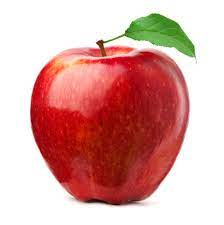
\includegraphics[scale=0.75]{../data/index.jpeg}
    \caption{apple}
    \end{figure}

    \section*{Discussion}

    \bibliographystyle{plain}

    \bibliography{ReportBiblio}
\end{document}